\documentclass[
	a4paper,
	oneside,
	BCOR = 10mm,
	DIV = 12,
	12pt,
	headings = normal,
]{scrartcl}

%%% Length calculations
\usepackage{calc}
%%%

%%% Support for color
\usepackage{xcolor}
\definecolor{lightblue}{HTML}{03A9F4}
\definecolor{red}{HTML}{F44336}
%%%

%%% Including graphics
\usepackage{graphicx}
%%%

%%% Font selection
\usepackage{fontspec}

\setromanfont{STIX Two Text}[
	SmallCapsFeatures = {LetterSpace = 8},
]

\setsansfont{IBM Plex Sans}[
	Scale = MatchUppercase,
]

\setmonofont{IBM Plex Mono}[
	Scale = MatchUppercase,
]
%%%

%%% Math typesetting
\usepackage{amsmath}

\usepackage{unicode-math}
\setmathfont{STIX Two Math}
%%%

%%% List settings
\usepackage{enumitem}
\setlist[enumerate]{
	label*      = {\arabic*.},
	leftmargin  = *,
	labelindent = \parindent,
	topsep      = 1\baselineskip,
	parsep      = 0\baselineskip,
	itemsep     = 1\baselineskip,
}

\setlist[itemize]{
	label*      = {—},
	leftmargin  = *,
	labelindent = \parindent,
	topsep      = 1\baselineskip,
	parsep      = 0\baselineskip,
	itemsep     = 1\baselineskip,
}

\setlist[description]{
	font        = {\rmfamily\upshape\bfseries},
	topsep      = 1\baselineskip,
	parsep      = 0\baselineskip,
	itemsep     = 0\baselineskip,
}

%%%

%%% Structural elements typesetting
\setkomafont{pagenumber}{\rmfamily}
\setkomafont{disposition}{\rmfamily\bfseries}

% Sectioning
\RedeclareSectionCommand[
	beforeskip = -1\baselineskip,
	afterskip  = 1\baselineskip,
	font       = {\normalsize\bfseries\scshape},
]{section}

\RedeclareSectionCommand[
	beforeskip = -1\baselineskip,
	afterskip  = 1\baselineskip,
	font       = {\normalsize\bfseries\itshape},
]{subsection}

\RedeclareSectionCommand[
	beforeskip = -1\baselineskip,
	afterskip  = 1\baselineskip,
	font       = {\normalsize\bfseries},
]{subsubsection}

\RedeclareSectionCommand[
	beforeskip = -1\baselineskip,
	afterskip  = -0.5em,
	font       = {\normalsize\mdseries\scshape\addfontfeatures{Letters = {UppercaseSmallCaps}}},
]{paragraph}
%%%

%%% Typographic enhancements
\usepackage{microtype}
%%%

%%% Language-specific settings
\usepackage{polyglossia}
\setmainlanguage{ukrainian}
\setotherlanguages{english}
%%%

%%% Captions
\usepackage{caption}
\usepackage{subcaption}

%\DeclareCaptionLabelFormat{closing}{#2)}
%\captionsetup[subtable]{labelformat = closing}

%\captionsetup[subfigure]{labelformat = closing}

\captionsetup[table]{
	aboveskip = 0\baselineskip,
	belowskip = 0\baselineskip,
}

\captionsetup[figure]{
	aboveskip = 1\baselineskip,
	belowskip = 0\baselineskip,
}

\captionsetup[subfigure]{
	labelformat = simple,
	labelformat = brace,
}
%%%

%%% Hyphenated ragged typesetting
\usepackage{ragged2e}
%%%

%%% Table typesetting
\usepackage{booktabs}
\usepackage{longtable}

\usepackage{multirow}

\usepackage{array}
\newcolumntype{v}[1]{>{\RaggedRight\arraybackslash\hspace{0pt}}p{#1}}
\newcolumntype{b}[1]{>{\Centering\arraybackslash\hspace{0pt}}p{#1}}
\newcolumntype{n}[1]{>{\RaggedLeft\arraybackslash\hspace{0pt}}p{#1}}
%%%

%%% Drawing
\usepackage{tikz}
\usepackage{tikzscale}
\usetikzlibrary{positioning}
\usetikzlibrary{arrows.meta} % Stealth arrow tips
%%%

%%% SI units typesetting
\usepackage{siunitx}
\sisetup{
	output-decimal-marker = {,},
	exponent-product      = {\cdot},
	inter-unit-product    = \ensuremath{{} \cdot {}},
	per-mode              = symbol,
}
%%%

%%% Links and hyperreferences
\usepackage{hyperref}
\hypersetup{
	bookmarksnumbered = true,
	colorlinks      = false,
	linkbordercolor = red,
	urlbordercolor  = lightblue,
	pdfborderstyle  = {/S/U/W 1.5},
}
%%%

%%% Length adjustments
% Set baselineskip, default is 14.5 pt
\linespread{1.068966} % ~15.5 pt
\setlength{\emergencystretch}{1em}
\setlength{\parindent}{1.5em}
\newlength{\gridunitwidth}
\setlength{\gridunitwidth}{\textwidth / 12}
%%%

%%% Custom commands
\newcommand{\allcaps}[1]{{\addfontfeatures{LetterSpace = 8, Kerning = Off}#1}}
%%%

\begin{document}

\begin{titlepage}
		\begin{center}
			Міністерство освіти і науки України\\
			Національний авіаційний університет\\
			Навчально-науковий інститут комп'ютерних інформаційних технологій\\
			Кафедра комп'ютеризованих систем управління

			\vspace{\fill}
				Лабораторна робота №2\\
				Частина 1\\
				з дисципліни «Телекомунікаційні~технології комп'ютерних~мереж»\\
				на тему «Кабелі комп'ютерних мереж на основі витої пари»\\

			\vspace{\fill}

			\begin{flushright}
				Виконав:\\
				студент \allcaps{ННІКІТ}\\
				групи СП-325\\
				Клокун В.\,Д.\\
				Перевірив:\\
				Пушкін Ю.\,О.
			\end{flushright}

			Київ 2018
		\end{center}
	\end{titlepage}

	\section{Мета роботи}
		Ознайомитись з видами, конструкцією з характеристиками кабелю вита пара; процесами, які відбуваються в кабелі під час передачі сигналів, параметрами кабелів, які використовуються при прокладенні ліній зв'язку локальних мереж.

	\section{Контрольні запитання}
		\subsection{Дайте визначечння понять «вита пара», «кабель вита пара»}
			Витою парою або~провідником вита пара еазивають два провідники, покриті ізоляціжю і~скручені в~джгут з~регулярним кроком. 

			Кабелі вита пара~— це такі кабелі, які складаються з~декількох витих пар, розміщених в~загальній захисній оболонці.

		\subsection{З якою метою скручують провідники?}
			Скрутка проводів дозволяє зменшити індуктивність проводів, яка призводить до~обмеження технічної швидкості. Крім того, скрутка сприяє зменшенню електричних завад, що~наводяться сусідніми парами і~зовнішніми джерелами.

		\subsection{Опишіть провідники витих пар}
			Провідники виготовляються з~мідного дроту і~можуть бути одножильними~(\textenglish{solid}~— монолітними) або багатожильними~(\textenglish{multiple-strand}). Багатожильні провідники є~джгутами, сплетеними з~мідних або луджених мідних тоненьких дротинок. Монолітна жила витої пари має діаметр в~межах \textenglish{\allcaps{AWG}}~26-22~(\SI{0.404}{\milli\meter}—\SI{0.643}{\milli\metre}, найбільш популярний~— \SI{0.511}{\milli\metre}), а~багатожильний провідник скручується з~дротинок діаметром~\SI{0.18}{\milli\metre}.

		\subsection{Опишіть ізоляційну і захисну оболонки кабелю «вита пара»}
			Електричну ізоляцію провідників витих пар виготовляють з полівінілхлориду, для витих пар вищих категорій — з поліпропілену або тефлону. Товщина шару ізоляції жил складає $0{,}2 – 0{,}6$~\si{\milli\metre}, причому стандарт~\textenglish{\allcaps{ISO/IEC}~118801} рекомендує, щоб діаметр провідника в ізоляції не перевищував~\SI{1.6}{\milli\metre}.

			Від механічних і кліматичних впливів провідники кабелю захищає зовнішня діелектрична оболонка товщиною~\SI{0.5}{\milli\metre}–\SI{0.8}{\milli\metre}. Як правило її виготовляють з поліетилену або полівінилхлориду з додаванням крейди для придання крихкості, щоб легше було наламувати оболонку у місці розрізу. Поліетилен найбільш технологічний і відносно дешевий матеріал, має достатню механічну міцність і вологостійкість, що важливо для кабелів зовнішнього прокладання, але він підтримує горіння.

			Полівінилхлорид не підтримує горіння, але у процесі виділяє отруйні речовини, тому використовують спеціальну марку кабелів \textenglish{\allcaps{LSZH/LS0H}~(Low Smoke Zero Halogen)}. Такий кабель практично не горить, не містить галогени і при сильному горінні виділяє мало диму, однак і коштує на 20-30\% дорожче полівінілхлоридових. 

		\subsection{Що означає абревіатура \textenglish{\allcaps{AWG?}}}
			\textenglish{American Wire Gage}~— одиниці американського калібру дроту, виміри якого базуються на дюймах.

		\subsection{Опишіть схему симетричного електричного кола, утвореного провідниками витої пари}
			Вита пара утворює лінію передачі сигналу за схемою симетричного електричного кола~(рис.~\ref{fig:twisted-pair-schematic}). 
			\begin{figure}[!htbp]
				\centering
				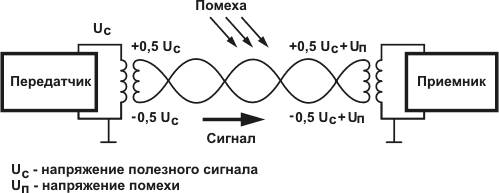
\includegraphics[height = 8\baselineskip]{./assets/y03s01-telecom-lab-02-01-p01.jpg}
				\caption{Схема симетричного електричного кола витої пари}
				\label{fig:twisted-pair-schematic}
			\end{figure}
			Приймач і передавач не мають гальванічного зв'язку один з одним внаслідок використання узгоджуючих трансформаторів. Передавач генерує сигнал~$U_{t\text{с}}$, який наводить на вихідних клемах вторинної обмотки протифазні сигнали~$+0{,}5~U_{\text{с}}$ і~$−0{,}5~U_{\text{с}}$. Тоді приймач реагує на різницю сигналів на обох провідниках на вхідних клемах первинної обмотки трансформатора приймача. 

			Напруги~$U_{\text{з}}$, наведені в результаті індукції і подані на первинну обмотку приймаючого трансформатора, є рівними за значенням і протилежними за знаком. В результаті різниця наведених потенціалів на вхідній обмотці дорівнює нулю і на вторинній обмотці трансформатора формується напруга сигналу.


		\subsection{Що означають поняття «швидкість поширення сигналу» і «затримка поширення»}
			Швидкість поширення сигналу~(\textenglish{nominal velocity of propagation, \allcaps{NVP}}) визначається як відношення швидкості руху сигналу в провіднику до швидкості світла у вакуумі.

			Затримка сигналу~(\textenglish{delay}) є похідною від швидкості поширення сигналу, вимірюється в~\si{\nano\second\per100\metre}.

		\subsection{Що означають поняття «поверхневий ефект» і «індуктивне наведення струму»?}
			Суть поверхневого ефекту полягає в тому, що внаслідок самоіндукції струм у провіднику витісняється на його поверхню, тобто зменшується ефективний переріх провідника і збільшується його активний опір.

			Індуктивне наведення струму полягає в тому, що внаслідок проходження високочастотного струму в одному провіднику за рахунок індукції наводиться вихрові струми в провідниках, розміщених поряд, і екранній оболонці, тобто у них створюється потенціал~(напруга)~завади~$U_{\text{з}}$. Зі збільшенням частоти сигналу енергія наведених струмів зростає і збільшується її вплив на сигнал.

		\subsection{Що означає поняття «перехресні індуктивні наведення»?}
			Перехресні індуктивні наведення означають, що високочастотний сигнал в одній парі індукує (наводить) струми і напруги, яка пропорційна потужності сигналу і створює перехідні завади (шуми), в інших парах кабелю.

		\subsection{Поясніть, що означають поняття «активний опір», «реактивний опір», «імпеданс»}
			Активний опір показує опір провідника постійному струму і залежить від параметрів даного провідника. Реактивний опір показує уявну частину імпедансу. Імпеданс характеризує опір провідника змінному струму і залежить від частоти струму. Імпеданс є повним опором провідника.

		\subsection{Поясніть причини затухання сигналу в кабелі вита пара і який параметр характеризує затухання}
			Затухання сигналу виникає через неоднорідність середовища провідника кабелю. Параметр, який характеризує затухання, називається коефіцієнтом затухання, і показує затухання на одиницю довжини (як правило, вимірюється у \si{\deci\bel\per100\metre}).
			\[
				A_x = 10 \log \left(\frac{\SI{1}{\milli\watt}}{P_x}\right).
			\]

		\subsection{Що характеризують параметри \textenglish{\allcaps{NEXT}, \allcaps{FEXT}, \allcaps{ELFEXT}}}
		Параметр \textenglish{\allcaps{NEXT}}~(перехресні наведення на~ближньому кінці) дозволяє оцінити стійкість кабеля у випадку, коли наведення утворюється в результаті дії сигналу, який генерується передавачем, підключеним до однієї з сусідніх пар на тому ж кінці кабелю, на якому працює приймач, підключений до підверженої пари. 
		
		\textenglish{\allcaps{FEXT}}~(перехресні наведення на~дальньому кінці)~— це параметр, який дозволяє оцінити стійкість кабеля до наведень у випадку, коли передавач і приймач підключені до різних кінців кабелів. 

		Параметр \textenglish{\allcaps{ELFEXT}} є значенням \textenglish{\allcaps{FEXT}}, приведеним до рівня корисного сигналу на дальньому кінці кабелю. Цей параметр враховує затухання на дальному кінці пари, сигнал, якій наводить індукцію в досліджуваній парі.

	\section{Висновок}
		Ознайомились з видами, конструкцією з характеристиками кабелю вита пара; процесами, які відбуваються в кабелі під час передачі сигналів, параметрами кабелів, які використовуються при прокладенні ліній зв'язку локальних мереж.

\end{document}
